%% LyX 2.1.4 created this file.  For more info, see http://www.lyx.org/.
%% Do not edit unless you really know what you are doing.
\documentclass[english,spanish]{article}
\usepackage[T1]{fontenc}
\usepackage[latin9]{inputenc}
\usepackage{geometry}
\geometry{verbose,tmargin=3cm,bmargin=3cm,lmargin=3cm,rmargin=3cm}
\usepackage{color}
\usepackage{babel}
\addto\shorthandsspanish{\spanishdeactivate{~<>}}

\usepackage{float}
\usepackage{amsmath}
\usepackage{amsthm}
\usepackage{graphicx}
\usepackage[unicode=true,pdfusetitle,
 bookmarks=true,bookmarksnumbered=true,bookmarksopen=true,bookmarksopenlevel=10,
 breaklinks=true,pdfborder={0 0 1},backref=false,colorlinks=true]
 {hyperref}
\hypersetup{
 linkcolor=blue, urlcolor=blue}

\makeatletter
%%%%%%%%%%%%%%%%%%%%%%%%%%%%%% Textclass specific LaTeX commands.
\numberwithin{equation}{section}
\numberwithin{figure}{section}

\makeatother

\usepackage{listings}
\addto\captionsenglish{\renewcommand{\lstlistingname}{Listing}}
\addto\captionsspanish{\renewcommand{\lstlistingname}{Listado de c�digo}}
\renewcommand{\lstlistingname}{Listado de c�digo}

\begin{document}

\author{bTactic - open source \& cloud solutions\\
\href{http://www.btactic.com}{http://www.btactic.com}}


\title{bSmtp zimlet - Manual del administrador}

\maketitle
\tableofcontents{}


\section{\label{sec:Instal=0000B7lar-el-Zimlet}Instalar el zimlet}

Para instalar el zimlet desde el servidor tenemos que abrir una terminal
al servidor con el usuario zimbra y ejecutar los siguientes comandos:

\begin{lstlisting}[tabsize=4,frame=single]
$ su - zimbra
$ zmzimletctl deploy <ruta al fichero com_btactic_bsmtp.zip>
\end{lstlisting}
Para poder instalar el zimlet desde la terminal tenemos que haber
descargado previamente el zip que contiene el zimlet en el servidor.\\
\\
Este es un ejemplo del resultado de la ejecuci�n de los comandos descritos
anteriormente:

\begin{lstlisting}[tabsize=4,frame=single]
$ zmzimletctl deploy /home/btactic/com_btactic_bsmtp.zip
[] INFO: Deploying Zimlet com_btactic_bsmtp in LDAP.
[] INFO: Installing Zimlet com_btactic_bsmtp on this host.
[] INFO: Upgrading Zimlet com_btactic_bsmtp to 1.0
[] INFO: Adding Zimlet com_btactic_bsmtp to COS default
[] INFO: Enabling Zimlet com_btactic_bsmtp
\end{lstlisting}



\section{Post instalaci�n}

Para que el zimlet funcione correctamente se han de ejecutar los siguientes
comandos desde la terminal del servidor de Zimbra\emph{:}

\begin{lstlisting}[tabsize=4,frame=single]
$ su - zimbra
$ zmprov modifyServer $(zmhostname) zimbraZimletJspEnabled TRUE
$ zmcontrol restart
\end{lstlisting}
En el caso de disponer de una instalaci�n multi-server de Zimbra se
debe ejecutar en todos los servidores de mailbox.


\section{\label{sec:3 Activar i desactivar el Zimlet}Activar/desactivar el
zimlet}

Para modificar el estado del zimlet (activado/desactivado) hay que
acceder a la configuraci�n de los zimlets. Veamos el proceso a seguir:
\begin{enumerate}
\item Como se puede observar en la figura \ref{fig:Pas 1} el primer paso
es entrar en la consola de administraci�n de Zimbra y seguidamente
a la pesta�a \textbf{\emph{Configurar}}.


\begin{figure}[H]
\begin{centering}
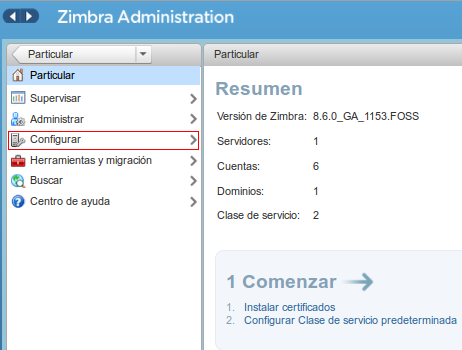
\includegraphics[clip,scale=0.5]{screenshots_admin_es/Step1-1}
\par\end{centering}

\caption{\selectlanguage{english}%
\label{fig:Pas 1}\foreignlanguage{spanish}{Ventana inicial de la
consola de administraci�n, pesta�a \textbf{\emph{Configurar}}}\selectlanguage{spanish}%
}
\end{figure}


\item Seguidamente ir al apartado \textbf{\emph{Zimlets }}(ver figura \ref{fig:Pas 2}).


\begin{figure}[H]
\begin{centering}
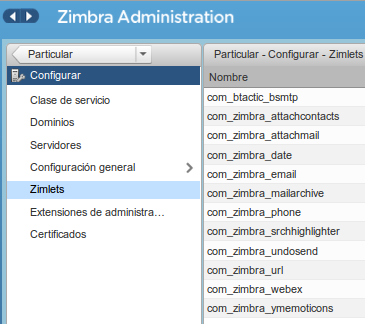
\includegraphics[clip,scale=0.5]{screenshots_admin_es/Step1-2}
\par\end{centering}

\caption{\selectlanguage{english}%
\label{fig:Pas 2}\foreignlanguage{spanish}{Panel de configuraci�n,
apartado \textbf{\emph{Zimlets}}}\selectlanguage{spanish}%
}
\end{figure}


\end{enumerate}
Una vez nos encontramos en el panel de configuraci�n de los zimlets,
tenemos que clicar con el bot�n derecho del rat�n encima de \textbf{\emph{com\_btactic\_bsmtp}}.
Se desplegar� un men� del cual tenemos que clicar la opci�n \textbf{\emph{Estado
de conmutaci�n}} (ver figura \ref{fig:Activar i desactivar zimlet}).\\
\\
Este procedimiento provocar� que el estado del zimlet pase de activado
a desactivado o viceversa. Podemos saber en que estado se encuentra
el zimlet fij�ndonos en la columna estado.\\
\\
Cabe destacar que para que el zimlet est� disponible el estado tiene
que ser \textbf{\emph{Activado}}, en caso contrario (estado \textbf{\emph{Desactivado}})
no estar� disponible.

\begin{figure}[H]
\begin{centering}
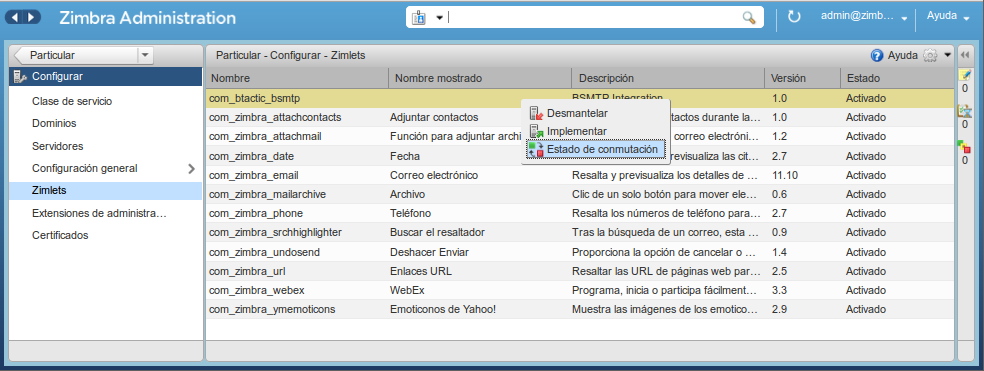
\includegraphics[clip,scale=0.5]{screenshots_admin_es/Step3-1}
\par\end{centering}

\caption{\label{fig:Activar i desactivar zimlet}Activar/desactivar un zimlet}
\end{figure}



\section{Habilitar el zimlet en la clase de servicio del usuario}

Para habilitar el zimlet en la clase de servicio del usuario tenemos
que entrar en la consola de administraci�n, pesta�a \textbf{\emph{Configurar
}}(m�s detalles en el paso 1 del apartado \ref{sec:3 Activar i desactivar el Zimlet})
y una vez all�, tenemos que seguir los pasos descritos a continuaci�n:
\begin{enumerate}
\item En el men� de la izquierda clicar \textbf{\emph{Clase de servicio}}
y seleccionar la clase de servicio en la que queremos habilitar el
zimlet (ver figura \ref{fig:Configuraci=0000F3 classe de servei}).


\begin{figure}[H]
\begin{centering}
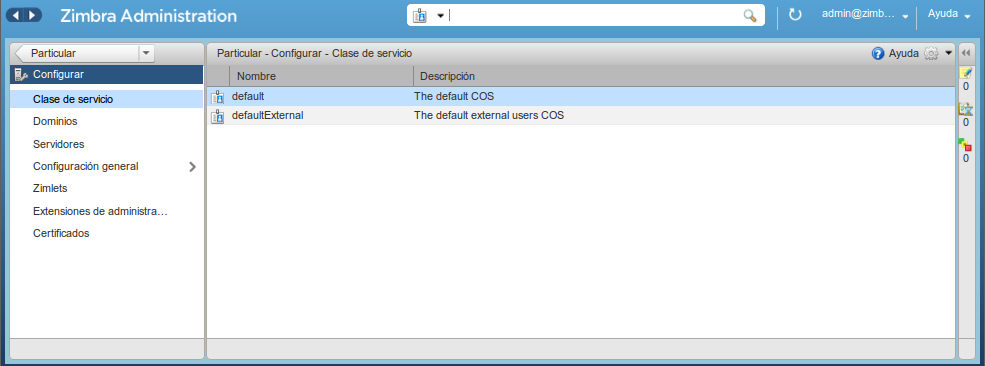
\includegraphics[clip,scale=0.5]{screenshots_admin_es/Step4-1}
\par\end{centering}

\caption{\label{fig:Configuraci=0000F3 classe de servei}Configuraci�n clase
de servicio}
\end{figure}


\item Una vez nos encontramos en la clase de servicio que queremos editar,
tenemos que clicar el icono 
\includegraphics[scale=0.65]{screenshots_admin_es/icon_config}
situado en la parte superior derecha de la pantalla y seleccionar
la opci�n \textbf{\emph{Editar}}\emph{ }(ver figura \ref{fig:Editar classe de servei})\emph{.}


\begin{figure}[H]
\begin{centering}
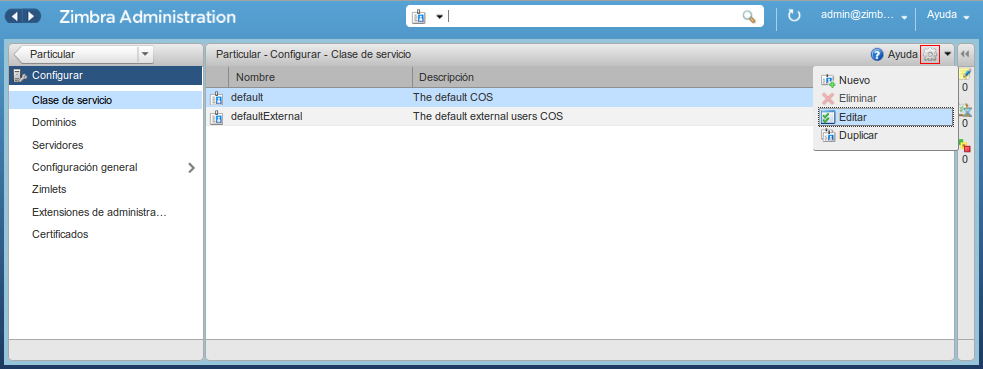
\includegraphics[clip,scale=0.5]{screenshots_admin_es/Step4-2}
\par\end{centering}

\caption{\label{fig:Editar classe de servei}Editar clase de servicio}
\end{figure}


\item Una vez nos encontramos en la configuraci�n de la clase de servicio
que queremos editar, tenemos que ir a la secci�n \textbf{\emph{Zimlets}}
del panel de la izquierda y una vez all� editar la configuraci�n de
\textbf{\emph{com\_btactic\_bsmtp }}siguiendo estos criterios:

\begin{itemize}
\item \textbf{obligatorio }activar� el zimlet y har� que el zimlet sea invisible
en la preferencia del cliente web. Por lo tanto, el usuario no podr�
deshabilitar el zimlet.
\item \textbf{activado} y \textbf{desactivado}\textbf{\emph{ }}solo definen
el estado predeterminado del zimlet. Los usuarios lo pueden habilitar
y deshabilitar.
\end{itemize}

Ver la figura \ref{fig:Configuraci=0000F3 dels Zimlets a la classe de servei}.


\begin{figure}[H]
\begin{centering}
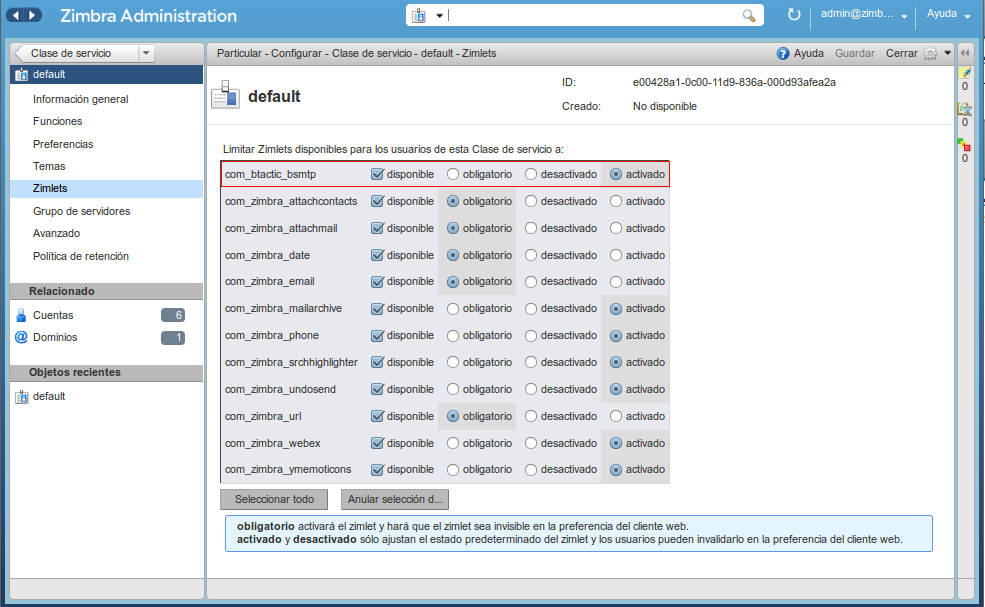
\includegraphics[clip,scale=0.5]{screenshots_admin_es/Step4-3}
\par\end{centering}

\caption{\label{fig:Configuraci=0000F3 dels Zimlets a la classe de servei}Configuraci�n
del los zimlets en la clase de servicio}
\end{figure}


\end{enumerate}

\section{C�digo fuente del zimlet}

El c�digo fuente y las distribuciones del zimlet est�n disponibles
en \href{https://github.com/btactic/bsmtp}{https://github.com/btactic/bsmtp}
\end{document}
